\chapter{具体需求}


\section{功能需求}

本子章节详细列出了我们产品的各个功能点的输入怎样被转换成输出,
	并描述了软件必须执行的基本动作。

\subsection{R.CLOUDMUSIC.SYS.001客户端启动}
\subsubsection{介绍}
	这是在客户端启动时,我们需要处理的功能点,包括:
	\begin{itemize}
		\item 检查更新,若有更新,应当通知用户;
		\item 进行主页初始化(R.CLOUDMUSIC.APP.001),显示主页(Home)界面的信息,供用户使用;
		\item 进行账户自动登录(R.CLOUDMUSIC.USER.001),如果上次关闭时已登录,
			则使用上一次的登录信息尝试自动登录;
		\item 进行音乐集列表同步(R.CLOUDMUSIC.SHOP.001),如果登录成功,
			需要对用户主页显示的音乐集做云同步;
		\item 对于部分客户端类型,展示APP开屏,用于等待初始化时的信息展示,
			也可展示广告;
	\end{itemize}
\subsubsection{输入}
	\begin{itemize}
		\item \textbf{输入来源}:客户端所在系统或浏览器;
		\item \textbf{内容}:用户打开了对应程序或网页,系统或浏览器发出的响应需求请求;
		\item \textbf{有效输入范围}:需判定为合法的请求;
	\end{itemize}
\subsubsection{处理}
	\begin{enumerate}
		\item 检测输入有效性,对于软件客户端,检测请求来源和格式是否符合标准,
			对于网页客户端,检测请求是否合法,否则请传输错误网页或特定网页
			(如404网页);
		\item 检查更新,若有更新,应当通知用户,若用户同意升级,则进行升级
			(详见R.CLOUDMUSIC.SYS.003);
		\item 进行主页初始化,详细请见 R.CLOUDMUSIC.APP.001;
		\item 若上次关闭时,用户登录了账户且网络已连接,则使用上次登录时的账户信息与
			缓存的登陆信息,尝试进行自动登陆(登录功能请见R.CLOUDMUSIC.USER.001)
			若成功,则进行音乐集的云同步(详细功能需求请见XXXX)
			若不成功,需要告知用户,进行重新手动登陆,并展示缓存在本地的主页配置;
		\item 如果是移动客户端,在以上过程中,需要使用APP开屏来在加载期间向用户展示
			歌曲推荐内容或广告,展示的内容是事先保存的,而在展示的过程中,也要
			联网向服务器查询同步下一次要向用户展示的APP开屏图片;
	\end{enumerate}
	\noindent 异常处理:
	\begin{enumerate}
		\item \textbf{网络错误}:不进行自动登陆操作、不进行APP开屏同步数据、不进行音乐集同步;
		\item \textbf{登录失败}:通知用户重新登录、不进行音乐集同步;
		\item \textbf{初始化失败}:返回错误信息;
	\end{enumerate}
\subsubsection{输出}
\begin{itemize}
	\item \textbf{输出位置}:响应系统的请求或响应浏览器的请求;
	\item \textbf{内容}:通过具体响应,告知启动初始化完成;
	\item \textbf{有效输出范围}:按照系统响应请求的方式或者网络服务发出响应报文的
		正确格式决定相关输出;
	\item \textbf{错误消息}:返回错误信息,具体方式按照系统响应请求的方式
		或者网络服务发出响应报文的格式;
\end{itemize}

\subsection{R.CLOUDMUSIC.SYS.002客户端关闭}
\subsubsection{介绍}
	这是在客户端关闭时,我们需要处理的功能点,包括:
	\begin{itemize}
		\item 检查是否有下载任务,若有,询问用户;
		\item 暂停所有的下载服务以及流服务;
		\item 最后进行一次同步数据(R.CLOUDMUSIC.SHOP.001);
		\item 关闭程序
	\end{itemize}
\subsubsection{输入}
	\begin{itemize}
		\item \textbf{输入来源}:客户端所在系统或浏览器;
		\item \textbf{内容}:用户或系统关闭了对应程序或网页,系统或浏览器发出的响应需求请求;
		\item \textbf{有效输入范围}:需判定为合法的请求;
	\end{itemize}
\subsubsection{处理}
	\begin{enumerate}
		\item 检测输入有效性,对于软件客户端,检测请求来源和格式是否符合标准,
			对于网页客户端,检测请求是否是合法的断开连接请求;
		\item 检测是否有正在运行的下载服务,如果有,询问用户是否任要关闭;
		\item 断开下载服务(如果有);
		\item 断开流数据服务(如果有);
	\end{enumerate}
	\noindent 异常处理:
	\begin{enumerate}
		\item \textbf{网络错误}:告知用户同步失败,询问是否重试,
			若用户选择重试,则重试,否则,放弃同步;
	\end{enumerate}
\subsubsection{输出}
\begin{itemize}
	\item \textbf{输出位置}:响应系统的请求或响应浏览器的请求;
	\item \textbf{内容}:通过具体响应,告知关闭完成;
	\item \textbf{有效输出范围}:按照系统响应请求的方式或者网络服务发出响应报文的
		正确格式决定相关输出;
	\item \textbf{错误消息}:返回错误信息,具体方式按照系统响应请求的方式
		或者网络服务发出响应报文的格式;
\end{itemize}

\subsection{R.CLOUDMUSIC.SYS.003客户端升级}
\subsubsection{介绍}
	这是在客户端升级时(网页客户端不考虑),我们需要处理的功能点,包括:
	\begin{itemize}
		\item 向服务端请求更新所需的文件并校验升级文件;
		\item 应用升级并重启;
	\end{itemize}
\subsubsection{输入}
	\begin{itemize}
		\item \textbf{输入来源}:客户端;
		\item \textbf{内容}:用户主动要求升级或者同意了自动检测的升级请求;
		\item \textbf{有效输入范围}:需判定为合法的请求;
	\end{itemize}
\subsubsection{处理}
	\begin{enumerate}
		\item 检测输入有效性,检测请求来源和格式是否符合标准;
		\item 检测是否有正在运行的下载服务,如果有,询问用户是否任然要升级;
		\item 进行标准的关闭程序操作(详见R.CLOUDMUSIC.SYS.002);
		\item 启动升级程序,进行升级包下载,并向多个服务器请求校验信息;
		\item 进行文件校验;
		\item 按照程序预先设定的文件更新方式进行升级;
		\item 完成后,重启程序(详见R.CLOUDMUSIC.SYS.001);
	\end{enumerate}
	\noindent 异常处理:
	\begin{enumerate}
		\item \textbf{网络错误}:告知用户升级失败,询问是否重试,
			若用户选择重试,则重试,否则,放弃升级,直接重启原来的版本;
		\item \textbf{校验错误}:同\textbf{网络错误}的处理方式;
	\end{enumerate}
\subsubsection{输出}
\begin{itemize}
	\item \textbf{输出位置}:客户端;
	\item \textbf{内容}:通过具体响应,告知升级完成;
	\item \textbf{有效输出范围}:无限制(根据客户端的程序逻辑,不会产生非法响应);
	\item \textbf{错误消息}:返回错误信息,告知客户端升级失败的原因,并通过客户端告知用户;
\end{itemize}

\subsection{R.CLOUDMUSIC.USER.001用户登陆}
\subsubsection{介绍}
	这是在 收到用户登录请求 时,我们需要处理的功能点,包括:
	\begin{itemize}
		\item 检测登录的凭证是否合法;
		\item 返回结果并更新凭证信息;
	\end{itemize}
\subsubsection{输入}
	\begin{itemize}
		\item \textbf{输入来源}:客户端或网页浏览器;
		\item \textbf{内容}:请求来源、账户名称、登陆凭据(详见下述);
		\item \textbf{有效输入范围}:需判定为合法的登陆请求;
	\end{itemize}
	\noindent 其中,登陆凭据的具体内容可以为加密后的密码信息,或者是上一次登录后
		服务器传回的登陆凭据;
\subsubsection{处理}
	\begin{enumerate}
		\item 检测输入有效性,检测请求来源和格式是否符合标准;
		\item 检查登陆凭据的合法性,若为加密后的密码,解密后进行校验,若成功,进入下一步,
			否则产生校验失败的异常;若为上一次登录后服务器传回的登陆凭据,
			则检测其是否已超时或失效,若有效且合法,进入下一步,否则产生登录超时的异常。
		\item 生成登陆凭据,在服务器上记录该凭据;
		\item 返回凭据;
	\end{enumerate}
	\noindent 异常处理:
	\begin{enumerate}
		\item \textbf{校验失败}:返回校验信息失败错误的信息,客户端将请求用户重试
			或尝试找回密码;
		\item \textbf{登录超时}:返回登录超时的信息,客户端将请求用户手动登陆;
	\end{enumerate}
\subsubsection{输出}
\begin{itemize}
	\item \textbf{输出位置}:客户端或网页浏览器;
	\item \textbf{内容}:若成功,返回登录凭据(对于网页客户端,是Cookie),
		若失败,返回登陆失败的原因;
	\item \textbf{有效输出范围}:无限制(根据服务端的程序逻辑,不会产生非法响应);
	\item \textbf{错误消息}:返回错误信息,告知用户登陆失败的原因,并按照情况处理;
\end{itemize}

\subsection{R.CLOUDMUSIC.USER.002用户注册}
\subsubsection{介绍}
	这是在 收到用户注册请求 时,我们需要处理的功能点,包括:
	\begin{itemize}
		\item 检测注册的相关信息是否合法;
		\item 在用户数据库中添加用户相关信息;
		\item 返回结果;
	\end{itemize}
\subsubsection{输入}
	\begin{itemize}
		\item \textbf{输入来源}:客户端或网页浏览器;
		\item \textbf{内容}:请求来源、注册信息(详见下述);
		\item \textbf{有效输入范围}:需判定为合法的注册请求;
	\end{itemize}
	\noindent 其中,注册信息的具体内容包括:
	\begin{itemize}
		\item 用户名(Username) 
		\item 密码(Password) 
		\item 邮箱(Email) 
	\end{itemize}
\subsubsection{处理}
	\begin{enumerate}
		\item 检测输入有效性,检测请求来源和格式是否符合标准;
		\item 检查使用的用户名和邮箱是否在数据库中有重复,使用的字符和长度是否
			是符合要求的,若有重复或不合法,则返回相应失败信息;
		\item 检查使用的密码,是否过于简单,若是,则返回失败信息;
		\item 返回注册结果;
	\end{enumerate}
	\noindent 异常处理:
	\begin{enumerate}
		\item \textbf{用户名或邮箱不合法}:
		返回不合法情况的相关失败错误的信息,客户端将请求用户重新按照要求注册;
		\item \textbf{密码过于简单}:返回错误的信息,客户端将请求用户使用更复杂的密码;
	\end{enumerate}
\subsubsection{输出}
\begin{itemize}
	\item \textbf{输出位置}:客户端或网页浏览器;
	\item \textbf{内容}:若成功,返回成功信息,若失败,返回注册失败的原因;
	\item \textbf{有效输出范围}:无限制(根据服务端的程序逻辑,不会产生非法响应);
	\item \textbf{错误消息}:返回错误信息,告知用户注册失败的原因,并按照情况处理;
\end{itemize}

\subsection{R.CLOUDMUSIC.USER.003用户注销}
\subsubsection{介绍}
	这是在 响应用户注销 时,我们需要处理的功能点,包括:
	\begin{itemize}
		\item 在服务端记录注销的信息,无效化相关登陆凭据;
	\end{itemize}
\subsubsection{输入}
	\begin{itemize}
		\item \textbf{输入来源}:客户端或网页浏览器;
		\item \textbf{内容}:请求来源,注销的用户信息;
		\item \textbf{有效输入范围}:需判定为合法的登陆请求;
	\end{itemize}
\subsubsection{处理}
	\begin{enumerate}
		\item 检测输入有效性,检测请求来源和格式是否符合标准;
		\item 检查注销请求是否合法,用户名是否存在;
		\item 在服务器上无效化相应的用户登陆凭据;
		\item 返回结果;
	\end{enumerate}
	\noindent 异常处理:
	\begin{enumerate}
		\item \textbf{校验失败}:返回注销失败的信息,客户端将请求重试,放弃注销;
	\end{enumerate}
\subsubsection{输出}
\begin{itemize}
	\item \textbf{输出位置}:客户端或网页浏览器;
	\item \textbf{内容}:若成功,返回注销成功的信息,
		若失败,返回注销失败的原因;
	\item \textbf{有效输出范围}:无限制(根据服务端的程序逻辑,不会产生非法响应);
	\item \textbf{错误消息}:返回错误信息,告知用户注销失败的原因,并按照情况处理;
\end{itemize}

\subsection{R.CLOUDMUSIC.APP.001生成主页界面}
\subsubsection{介绍}
	这是在 生成主页(Home)界面 时,我们需要处理的功能点,包括:
	\begin{itemize}
		\item 生成主页界面的内容;
	\end{itemize}
\subsubsection{输入}
	\begin{itemize}
		\item \textbf{输入来源}:客户端或网页浏览器;
		\item \textbf{内容}:客户端的状态或者网页的状态(如网页尺寸等);
		\item \textbf{有效输入范围}:需判定为合法的请求;
	\end{itemize}
\subsubsection{处理}
	\begin{enumerate}
		\item 检测输入有效性,检测请求来源和格式是否符合标准;
		\item 生成界面元素,具体的界面要求,请参照小节\ref{ssec:ui};
		\item 返回完成的信息;
	\end{enumerate}
\subsubsection{输出}
\begin{itemize}
	\item \textbf{输出位置}:客户端或网页浏览器;
	\item \textbf{内容}:告知生成完成;
	\item \textbf{有效输出范围}:无限制(根据服务端的程序逻辑,不会产生非法响应);
	\item \textbf{错误消息}:正常情况下不会产生非法响应,若有,则应视为程序BUG;
\end{itemize}

\subsection{R.CLOUDMUSIC.APP.002生成音乐集界面}
\subsubsection{介绍}
	这是在 生成音乐集界面 时,我们需要处理的功能点,包括:
	\begin{itemize}
		\item 判定音乐集是否可以被查看;
		\item 生成音乐集界面的内容;
	\end{itemize}
\subsubsection{输入}
	\begin{itemize}
		\item \textbf{输入来源}:客户端或网页浏览器;
		\item \textbf{内容}:请求的音乐集ID以及用户登录凭证(可选);
		\item \textbf{有效输入范围}:需判定为合法的请求;
	\end{itemize}
\subsubsection{处理}
	\begin{enumerate}
		\item 检测输入有效性,检测请求来源和格式是否符合标准;
		\item 检测登陆凭据,若校验失败或登录超时,返回对应错误,不进入下一步;
		\item 检查音乐集ID是否存在,若不存在,返回对应错误,不进入下一步;
		\item 检查音乐集的可访问性,若为私密(private)音乐集,
			检查用户凭证对应的账户是否对其有查看权,若否,返回对应错误,不进入下一步;
		\item 生成音乐集界面元素,具体的界面要求,请参照小节\ref{ssec:ui};
		\item 返回完成的信息;
	\end{enumerate}
	\noindent 异常处理:
	\begin{enumerate}
		\item \textbf{登录信息失败}:返回登陆失败错误的信息,客户端将请求用户重登陆;
		\item \textbf{音乐集ID不存在}:返回音乐集不存在的信息,客户端将展示错误页面;
		\item \textbf{音乐集不可访问}:返回音乐集不可访问性的信息,
			客户端将展示无法访问私密音乐集页面,若没有登录,询问是否登陆;
	\end{enumerate}
\subsubsection{输出}
\begin{itemize}
	\item \textbf{输出位置}:客户端或网页浏览器;
	\item \textbf{内容}:若成功,返回 音乐集界面生成完成的信息 ,若失败,返回 失败的原因;
	\item \textbf{有效输出范围}:无限制(根据服务端的程序逻辑,不会产生非法响应);
	\item \textbf{错误消息}:返回错误信息,告知用户查看失败的原因,并按照情况处理;
\end{itemize}

\subsection{R.CLOUDMUSIC.APP.003生成音乐播放界面}
\subsubsection{介绍}
	这是在 生成音乐播放界面 时,我们需要处理的功能点,包括:
	\begin{itemize}
		\item 判定音乐是否可以被查看;
		\item 生成音乐播放界面的内容;
	\end{itemize}
\subsubsection{输入}
	\begin{itemize}
		\item \textbf{输入来源}:客户端或网页浏览器;
		\item \textbf{内容}:请求的音乐ID以及用户登录凭证(可选);
		\item \textbf{有效输入范围}:需判定为合法的请求;
	\end{itemize}
\subsubsection{处理}
	\begin{enumerate}
		\item 检测输入有效性,检测请求来源和格式是否符合标准;
		\item 检测登陆凭据,若校验失败或登录超时,返回对应错误,不进入下一步;
		\item 检查音乐ID是否存在,若不存在,返回对应错误,不进入下一步;
		\item 检查音乐的可访问性,若为付费的音乐,
			检查用户凭证对应的账户是否对其有播放权,
			若否或没有登录,检查该音乐是否允许试听,若可以,生成试听模式的界面,
			否则返回错误信息;
		\item 若具有播放权,生成完整播放界面;
		\item 具体的两种界面的要求,请参照小节\ref{ssec:ui};
		\item 返回完成的信息;
	\end{enumerate}
	\noindent 异常处理:
	\begin{enumerate}
		\item \textbf{登录信息失败}:返回登陆失败错误的信息,客户端将请求用户重登陆;
		\item \textbf{音乐ID不存在}:返回音乐不存在的信息,客户端将展示错误页面;
		\item \textbf{音乐不可访问}:返回音乐集不可访问性的信息,客户端提示是否要购买;
	\end{enumerate}
\subsubsection{输出}
\begin{itemize}
	\item \textbf{输出位置}:客户端或网页浏览器;
	\item \textbf{内容}:若成功,返回 音乐播放界面生成完成的信息 ,若失败,返回 失败的原因;
	\item \textbf{有效输出范围}:无限制(根据服务端的程序逻辑,不会产生非法响应);
	\item \textbf{错误消息}:返回错误信息,告知用户尝试进入播放界面失败的原因,
		并按照情况处理;
\end{itemize}

\subsection{R.CLOUDMUSIC.APP.004生成音乐推荐界面}
\subsubsection{介绍}
	这是在 生成音乐推荐界面 时,我们需要处理的功能点,包括:
	\begin{itemize}
		\item 判定用户的登录状态;
		\item 生成音乐推荐界面的内容;
	\end{itemize}
\subsubsection{输入}
	\begin{itemize}
		\item \textbf{输入来源}:客户端或网页浏览器;
		\item \textbf{内容}:请求的来源以及用户登录凭证(可选);
		\item \textbf{有效输入范围}:需判定为合法的请求;
	\end{itemize}
\subsubsection{处理}
	\begin{enumerate}
		\item 检测输入有效性,检测请求来源和格式是否符合标准;
		\item 检测登陆凭据,若校验失败或登录超时,返回对应错误,不进入下一步;
		\item 向服务器请求个性化推荐以及音乐排名等信息,如果没有登录,
			则仅仅生成音乐排名的信息,不生成个性化内容;
		\item 生成音乐推荐界面的内容,具体的界面要求,请参照小节\ref{ssec:ui};
		\item 返回完成的信息;
	\end{enumerate}
	\noindent 异常处理:
	\begin{enumerate}
		\item \textbf{登录信息失败}:返回登陆失败错误的信息,客户端将请求用户重登陆;
		\item \textbf{网络访问}:返回网络错误的信息,客户端提示无法查看,
			请求用户检查网络状态;
	\end{enumerate}
\subsubsection{输出}
\begin{itemize}
	\item \textbf{输出位置}:客户端或网页浏览器;
	\item \textbf{内容}:若成功,返回 音乐推荐界面生成完成的信息 ,若失败,返回 失败的原因;
	\item \textbf{有效输出范围}:无限制(根据服务端的程序逻辑,不会产生非法响应);
	\item \textbf{错误消息}:返回错误信息,告知用户尝试进入推荐界面失败的原因,
		并按照情况处理;
\end{itemize}

\subsection{R.CLOUDMUSIC.APP.005生成账户界面}
\subsubsection{介绍}
	这是在 生成账户界面 时,我们需要处理的功能点,包括:
	\begin{itemize}
		\item 判定用户的登录状态;
		\item 生成对应的账户界面的内容;
	\end{itemize}
\subsubsection{输入}
	\begin{itemize}
		\item \textbf{输入来源}:客户端或网页浏览器;
		\item \textbf{内容}:请求的来源以及用户登录凭证(可选);
		\item \textbf{有效输入范围}:需判定为合法的请求;
	\end{itemize}
\subsubsection{处理}
	\begin{enumerate}
		\item 检测输入有效性,检测请求来源和格式是否符合标准;
		\item 若没有登陆,生成登陆界面,也要提供注册功能的入口;
		\item 检测登陆凭据,若校验失败或登录超时,返回对应错误,不进入下一步;
		\item 向服务器请求用户的数据;
		\item 生成用户的界面信息元素,具体的界面要求,请参照小节\ref{ssec:ui};
		\item 返回完成的信息;
	\end{enumerate}
	\noindent 异常处理:
	\begin{enumerate}
		\item \textbf{登录信息失败}:返回登陆失败错误的信息,客户端将请求用户重登陆;
		\item \textbf{网络访问}:返回网络错误的信息,客户端提示无法查看,
			请求用户检查网络状态;
	\end{enumerate}
\subsubsection{输出}
\begin{itemize}
	\item \textbf{输出位置}:客户端或网页浏览器;
	\item \textbf{内容}:若成功,返回 账户界面生成完成的信息 ,若失败,返回 失败的原因;
	\item \textbf{有效输出范围}:无限制(根据服务端的程序逻辑,不会产生非法响应);
	\item \textbf{错误消息}:返回错误信息,告知用户尝试进入账户界面失败的原因,
		并按照情况处理;
\end{itemize}

\subsection{R.CLOUDMUSIC.APP.006生成设置界面}
\subsubsection{介绍}
	这是在 生成设置界面 时,我们需要处理的功能点,包括:
	\begin{itemize}
		\item 生成设置界面的内容;
	\end{itemize}
\subsubsection{输入}
	\begin{itemize}
		\item \textbf{输入来源}:客户端或网页浏览器;
		\item \textbf{内容}:请求的来源;
		\item \textbf{有效输入范围}:需判定为合法的请求;
	\end{itemize}
\subsubsection{处理}
	\begin{enumerate}
		\item 检测输入有效性,检测请求来源和格式是否符合标准;
		\item 读取当前的用户设置信息;
		\item 生成对应的设置界面,请参照小节\ref{ssec:ui};
		\item 返回完成的信息;
	\end{enumerate}
\subsubsection{输出}
\begin{itemize}
	\item \textbf{输出位置}:客户端或网页浏览器;
	\item \textbf{内容}:若成功,返回 设置界面生成完成的信息 ,若失败,返回 失败的原因;
	\item \textbf{有效输出范围}:无限制(根据服务端的程序逻辑,不会产生非法响应);
	\item \textbf{错误消息}:理论上,该界面不应该发生错误,若有,则应当视为程序BUG;
\end{itemize}

\subsection{R.CLOUDMUSIC.MUSIC.001音乐播放控制}
\subsubsection{介绍}
	这是在 处于音乐播放的状态下 时,我们需要处理的功能点,包括:
	\begin{itemize}
		\item 响应一系列控制请求;
		\item 处理音乐的播放需求;
	\end{itemize}
\subsubsection{输入}
	\begin{itemize}
		\item \textbf{输入来源}:客户端或网页浏览器;
		\item \textbf{内容}:对音乐的控制请求,可能有以下具体需求:
		\begin{enumerate}
			\item 播放/暂停状态转换
			\item 下一曲/上一曲
			\item 进度条控制,需提供目标时间戳
			\item 播放的歌曲的跳转,需提供音乐ID
			\item 显示/隐藏歌词
			\item 切换列表播放模式
		\end{enumerate}
		\item \textbf{有效输入范围}:需要判断请求的合法性,具体如下:
		\begin{itemize}
			\item 对于 进度条控制,需检查时间戳的合法性;
			\item 对于 歌曲跳转,需要判断ID的合法性,以及是否有访问权; 
		\end{itemize}
	\end{itemize}
\subsubsection{处理}
	\begin{enumerate}
		\item 检测输入有效性,检测请求来源和格式是否符合标准;
		\item 对于输入的控制分别做处理:
		\begin{enumerate}
			\item \textbf{播放/暂停状态转换}:
				转换歌曲的播放或暂停状态;
			\item \textbf{下一曲/上一曲}:
				根据播放列表和列表播放模式,操作播放的音乐;
			\item \textbf{进度条控制,需提供目标时间戳}:
				首先判断时间戳输入的合法性(是否超出音乐时间的范围),
				然后跳转至该时间戳;
			\item \textbf{播放的歌曲的跳转,需提供音乐ID}:
				首先判断ID输入的合法性(是否是无效的ID或者没有访问权限),
				然后跳转至该时间戳;
			\item \textbf{显示/隐藏歌词}:
				切换歌词的展示状态
			\item \textbf{切换列表播放模式}:
				切换列表循环模式,在以下四项中循环切换:
					\begin{itemize}
						\item 列表顺序不循环播放
						\item 列表顺序循环播放
						\item 列表随机循环播放
						\item 单曲循环播放
					\end{itemize}
		\end{enumerate}
		\item 返回完成的信息;
	\end{enumerate}
\subsubsection{输出}
\begin{itemize}
	\item \textbf{输出位置}:客户端或网页浏览器;
	\item \textbf{内容}:若成功,返回操作完成的信息 ,若失败,返回失败的原因;
	\item \textbf{有效输出范围}:无限制(根据服务端的程序逻辑,不会产生非法响应);
	\item \textbf{错误消息}:返回错误信息,告知客户端操作失败的原因,
		但由于无效的操作不应该被发出,所以一般不会发生;
\end{itemize}

\subsection{R.CLOUDMUSIC.MUSIC.002音乐串流控制}
\subsubsection{介绍}
	这是在 处于音乐串流情形下 时,我们需要处理的功能点,包括:
	\begin{itemize}
		\item 连接服务器,验证串流可访问性;
		\item 处理音乐的串流需求;
	\end{itemize}
\subsubsection{输入}
	\begin{itemize}
		\item \textbf{输入来源}:客户端或网页浏览器;
		\item \textbf{内容}:对音乐的串流请求,包括:
		\begin{enumerate}
			\item 串流音乐的ID;
			\item 串流的目标时间戳;
			\item 串流的预缓存长度;
			\item 用户登陆凭据(可选);
		\end{enumerate}
		\item \textbf{有效输入范围}:需要判断请求的合法性,具体如下:
		\begin{itemize}
			\item 若有用户登陆凭据,需对其校验; 
			\item 需要判断ID的合法性,以及是否有访问权;
			\item 需判断时间戳的合法性; 
		\end{itemize}
	\end{itemize}
\subsubsection{处理}
	\begin{enumerate}
		\item 检测输入有效性,检测请求来源和格式是否符合标准;
		\item 若有用户登陆凭据,验证其合法性;
		\item 检查音乐ID的合法性,是否对当前的账户可访问,若
			是付费音乐,查看其是否可以试听,若可以,则进入试听模式,
			否则,拒绝串流请求;
		\item 检查时间戳合法性,检查预缓存长度是否超出限制;
		\item 返回对应的串流响应,建立串流连接;
	\end{enumerate}
\subsubsection{输出}
\begin{itemize}
	\item \textbf{输出位置}:客户端或网页浏览器;
	\item \textbf{内容}:若成功,返回对应的串流响应 ,若失败,返回失败的原因;
	\item \textbf{有效输出范围}:无限制(根据服务端的程序逻辑,不会产生非法响应);
	\item \textbf{错误消息}:按照系统响应请求的方式或者网络服务发出响应报文的
		正确格式决定相关输出;
\end{itemize}

\subsection{R.CLOUDMUSIC.MUSIC.003音乐下载控制}
\subsubsection{介绍}
	这是在 处理音乐下载请求 时,我们需要处理的功能点,包括:
	\begin{itemize}
		\item 连接服务器,验证音乐是否可下载;
		\item 处理音乐的下载请求;
	\end{itemize}
\subsubsection{输入}
	\begin{itemize}
		\item \textbf{输入来源}:客户端或网页浏览器;
		\item \textbf{内容}:对音乐的下载请求,包括:
		\begin{enumerate}
			\item 下载音乐的ID;
			\item 下载音乐的音质(可选);
			\item 用户登陆凭据(可选);
		\end{enumerate}
		\item \textbf{有效输入范围}:需要判断请求的合法性,具体如下:
		\begin{itemize}
			\item 若有用户登陆凭据,需对其校验; 
			\item 需要判断ID的合法性,以及是否有访问权;
		\end{itemize}
	\end{itemize}
\subsubsection{处理}
	\begin{enumerate}
		\item 检测输入有效性,检测请求来源和格式是否符合标准;
		\item 若有用户登陆凭据,验证其合法性;
		\item 检查音乐ID的合法性,是否对当前的账户可下载,
			否则,拒绝下载请求;
		\item 检查音质选项的合法性,若没有音质选项,使用默认设置;
		\item 返回对应的下载响应,建立下载连接;
	\end{enumerate}
\subsubsection{输出}
\begin{itemize}
	\item \textbf{输出位置}:客户端或网页浏览器;
	\item \textbf{内容}:若成功,返回对应的下载响应 ,若失败,返回失败的原因;
	\item \textbf{有效输出范围}:无限制(根据服务端的程序逻辑,不会产生非法响应);
	\item \textbf{错误消息}:按照系统响应请求的方式或者网络服务发出响应报文的
		正确格式决定相关输出;
\end{itemize}

\subsection{R.CLOUDMUSIC.SHOP.001购买音乐}
\subsubsection{介绍}
	这是在 处理音乐购买请求 时,我们需要处理的功能点,包括:
	\begin{itemize}
		\item 连接服务器,验证音乐的价格;
		\item 验证支付信息的真伪;
		\item 在数据库中修改账户的音乐访问权;
	\end{itemize}
\subsubsection{输入}
	\begin{itemize}
		\item \textbf{输入来源}:客户端或网页浏览器;
		\item \textbf{内容}:对音乐的购买请求,包括:
		\begin{enumerate}
			\item 购买音乐的ID的集合(可以一次购买多首);
			\item 用户登陆凭据;
			\item 用户完成支付的凭据(内部或外部);
		\end{enumerate}
		\item \textbf{有效输入范围}:需要判断请求的合法性,具体如下:
		\begin{itemize}
			\item 若有用户登陆凭据,需对其校验; 
			\item 需要判断ID的合法性;
		\end{itemize}
	\end{itemize}
\subsubsection{处理}
	\begin{enumerate}
		\item 检测输入有效性,检测请求来源和格式是否符合标准;
		\item 若有用户登陆凭据,验证其合法性;
		\item 检查音乐ID的合法性,是否已经在当前账户的已购买数据库中;
		\item 检查支付凭据的真伪;
		\item 在数据库中修改账户的音乐访问权;
		\item 返回对应的购买成功响应,提示用户是否开始下载对应音乐;
	\end{enumerate}
	\noindent 异常处理:
	\begin{enumerate}
		\item \textbf{登录信息失败}:返回登陆失败错误的信息,客户端将请求用户重登陆;
		\item \textbf{网络访问}:返回网络错误的信息,客户端提示用户检查网络状态;
	\end{enumerate}
\subsubsection{输出}
\begin{itemize}
	\item \textbf{输出位置}:客户端或网页浏览器;
	\item \textbf{内容}:若成功,返回对应的成功响应 ,若失败,返回失败的原因;
	\item \textbf{有效输出范围}:无限制(根据服务端的程序逻辑,不会产生非法响应);
	\item \textbf{错误消息}:按照系统响应请求的方式或者网络服务发出响应报文的
		正确格式决定相关输出;
\end{itemize}

\subsection{R.CLOUDMUSIC.SHOP.002购买订阅}
\subsubsection{介绍}
	这是在 处理订阅购买请求 时,我们需要处理的功能点,包括:
	\begin{itemize}
		\item 连接服务器,验证订阅的价格;
		\item 验证支付信息的真伪;
		\item 在数据库中修改账户的音乐访问权;
	\end{itemize}
\subsubsection{输入}
	\begin{itemize}
		\item \textbf{输入来源}:客户端或网页浏览器;
		\item \textbf{内容}:对订阅的购买请求,包括:
		\begin{enumerate}
			\item 用户登陆凭据;
			\item 购买订阅的时长;
			\item 是否自动续费;
			\item 用户完成支付的凭据(内部或外部);
		\end{enumerate}
		\item \textbf{有效输入范围}:需要判断请求的合法性,具体如下:
		\begin{itemize}
			\item 若有用户登陆凭据,需对其校验; 
		\end{itemize}
	\end{itemize}
\subsubsection{处理}
	\begin{enumerate}
		\item 检测输入有效性,检测请求来源和格式是否符合标准;
		\item 若有用户登陆凭据,验证其合法性;
		\item 检查支付凭据的真伪;
		\item 在数据库中修改账户的音乐访问权;
		\item 若要求自动续费,检查支付方式是否支持,
			若不支持,返回对应提示;
		\item 返回对应的购买成功响应,提示用户是否开始下载对应音乐;
	\end{enumerate}
	\noindent 异常处理:
	\begin{enumerate}
		\item \textbf{登录信息失败}:返回登陆失败错误的信息,客户端将请求用户重登陆;
		\item \textbf{网络访问}:返回网络错误的信息,客户端提示用户检查网络状态;
		\item \textbf{支付方式不支持}:返回对应错误的信息,客户端提示用户无法设置自动续费,
			并建议用户绑定新的支付方式;
	\end{enumerate}
\subsubsection{输出}
\begin{itemize}
	\item \textbf{输出位置}:客户端或网页浏览器;
	\item \textbf{内容}:若成功,返回对应的成功响应 ,若失败,返回失败的原因;
	\item \textbf{有效输出范围}:无限制(根据服务端的程序逻辑,不会产生非法响应);
	\item \textbf{错误消息}:按照系统响应请求的方式或者网络服务发出响应报文的
		正确格式决定相关输出;
\end{itemize}

\subsection{R.CLOUDMUSIC.SYNC.001数据同步上传}
\subsubsection{介绍}
	这是在 处理数据同步上传请求 时,我们需要处理的功能点,包括:
	\begin{itemize}
		\item 连接服务器,验证账户登陆凭据;
		\item 上传数据至服务器;
	\end{itemize}
\subsubsection{输入}
	\begin{itemize}
		\item \textbf{输入来源}:客户端或网页浏览器;
		\item \textbf{内容}:对数据同步上传请求,包括:
		\begin{enumerate}
			\item 用户登陆凭据;
			\item 当前时间;
			\item 变更的摘要;
		\end{enumerate}
		\item \textbf{有效输入范围}:需要判断请求的合法性,具体如下:
		\begin{itemize}
			\item 对于用户登陆凭据,需对其校验; 
			\item 对于时间,需验证是否为更新的数据; 
		\end{itemize}
	\end{itemize}
\subsubsection{处理}
	\begin{enumerate}
		\item 检测输入有效性,检测请求来源和格式是否符合标准;
		\item 若有用户登陆凭据,验证其合法性;
		\item 检查服务器中的数据库,检查是否有更新的数据;
		\item 根据数据变更的摘要,对服务器端做数据接收的准备;
		\item 建立服务器信道,返回响应,进行用户数据的上传;
	\end{enumerate}
	\noindent 异常处理:
	\begin{enumerate}
		\item \textbf{登录信息失败}:返回登陆失败错误的信息,客户端将请求用户重登陆;
		\item \textbf{网络访问}:返回网络错误的信息,客户端提示用户检查网络状态;
	\end{enumerate}
\subsubsection{输出}
\begin{itemize}
	\item \textbf{输出位置}:客户端或网页浏览器;
	\item \textbf{内容}:若成功,返回对应的成功响应 ,若失败,返回失败的原因;
	\item \textbf{有效输出范围}:无限制(根据服务端的程序逻辑,不会产生非法响应);
	\item \textbf{错误消息}:按照系统响应请求的方式或者网络服务发出响应报文的
		正确格式决定相关输出;
\end{itemize}

\subsection{R.CLOUDMUSIC.SYNC.002数据同步下载}
\subsubsection{介绍}
	这是在 处理数据同步下载请求 时,我们需要处理的功能点,包括:
	\begin{itemize}
		\item 连接服务器,验证账户登陆凭据;
		\item 下载数据至客户端;
	\end{itemize}
\subsubsection{输入}
	\begin{itemize}
		\item \textbf{输入来源}:客户端;
		\item \textbf{内容}:对数据同步下载请求,包括:
		\begin{enumerate}
			\item 用户登陆凭据;
			\item 请求数据的范围;
		\end{enumerate}
		\item \textbf{有效输入范围}:需要判断请求的合法性,具体如下:
		\begin{itemize}
			\item 对于用户登陆凭据,需对其校验; 
			\item 对于请求数据的范围,需验证是否已在数据库中; 
		\end{itemize}
	\end{itemize}
\subsubsection{处理}
	\begin{enumerate}
		\item 检测输入有效性,检测请求来源和格式是否符合标准;
		\item 若有用户登陆凭据,验证其合法性;
		\item 检查服务器中的数据库,检查是否请求数据的范围内的所有数据;
		\item 根据请求数据的范围,对服务器端做传输数据的准备;
		\item 建立服务器信道,返回响应,进行用户数据的下载;
	\end{enumerate}
	\noindent 异常处理:
	\begin{enumerate}
		\item \textbf{登录信息失败}:返回登陆失败错误的信息,客户端将请求用户重登陆;
		\item \textbf{网络访问}:返回网络错误的信息,客户端提示用户检查网络状态;
	\end{enumerate}
\subsubsection{输出}
\begin{itemize}
	\item \textbf{输出位置}:客户端或网页浏览器;
	\item \textbf{内容}:若成功,返回对应的成功响应 ,若失败,返回失败的原因;
	\item \textbf{有效输出范围}:无限制(根据服务端的程序逻辑,不会产生非法响应);
	\item \textbf{错误消息}:按照系统响应请求的方式或者网络服务发出响应报文的
		正确格式决定相关输出;
\end{itemize}

\section{性能需求}

\subsection{服务器响应需求}
\begin{enumerate}
	\item 对于响应R.CLOUDMUSIC.USER.001 $\sim$ 003的用户相关响应需求,
		以及R.CLOUDMUSIC.MUSIC.001 $\sim$ 003
		之中的服务器信道建立响应,需要在尽量少的时间内使用户得到
		响应,对于HTTP连接的响应,一般需要控制在500ms以下,
		不然会造成用户体验的下降;
	\item 对于R.CLOUDMUSIC.SHOP.001 $\sim$ 002中的支付相关的响应需求,
		由于可能向外部的支付机构查询相关订单的真伪,
		对于响应的延时,可以放宽要求至3500ms以下,
\end{enumerate}

\subsection{服务器带宽需求}
\begin{enumerate}
	\item 对于响应R.CLOUDMUSIC.MUSIC.001 $\sim$ 003
		之中的音乐播放、串流、下载服务,
		需要以较快的速度进行数据的传输。
	\item 由于音乐文件一般不大,对于播放、串流一般音质的音乐文件,
		我们一般只需要保证每用户稳定的100KB/s的下行速度;
	\item 对于下载请求,我们需要使用户尽快得到需要的文件,
		应尽可能保证每用户稳定的2.5MB/s的下行速度;
	\item 在服务器峰值时,应合理分配下载音乐使用的带宽,
		使得其他用户的播放、串流需求不受影响,
		这种情形下,应保证每用户稳定的512KB/s的下行速度;
\end{enumerate}

\subsection{数据库性能需求}
\begin{enumerate}
	\item 为了提供高并发访问,需要支持高并发的数据库或分布式数据库网络,
		每秒查询数在至少在100,000,000条以上。
	\item 为了保证不同音乐文件以及用户数据的存储,
		数据库应保证不少于10PB (10,000TB)的存储容量。
\end{enumerate}

\section{外部接口需求}
\subsection{用户接口}
\label{ssec:ui}

\subsubsection{PC客户端用户接口} % (fold)
本小节讲述在PC客户端上,用户接口应具有的设计需求。

\begin{enumerate}
	\item \textbf{要求的屏幕格式}:
		PC客户端支持大于$800 \times 600$ 分辨率的屏幕,并对根据屏幕大小以及系统
		设定的屏幕元素放大比例做自动适应;
	\item \textbf{使用方式}:
		对于一般的用户,我们的产品使用逻辑与一般的PC软件一致,
			用户不需要主动学习便可学会使用它,
		同时,我们也会在安装后附上使用说明书,来保证用户可以方便使用;
	\item \textbf{页面规划}: 
	\begin{itemize}
		\item 主页界面的用户接口设计,请参考图\ref{fig:desttop_home};
		\item 音乐播放界面的用户接口设计,请参考图\ref{fig:desttop_music};
		\item 音乐集查看界面的用户接口设计,请参考图\ref{fig:desttop_collection};
	\end{itemize}
\end{enumerate}

\begin{figure}[h!]
  \centering

  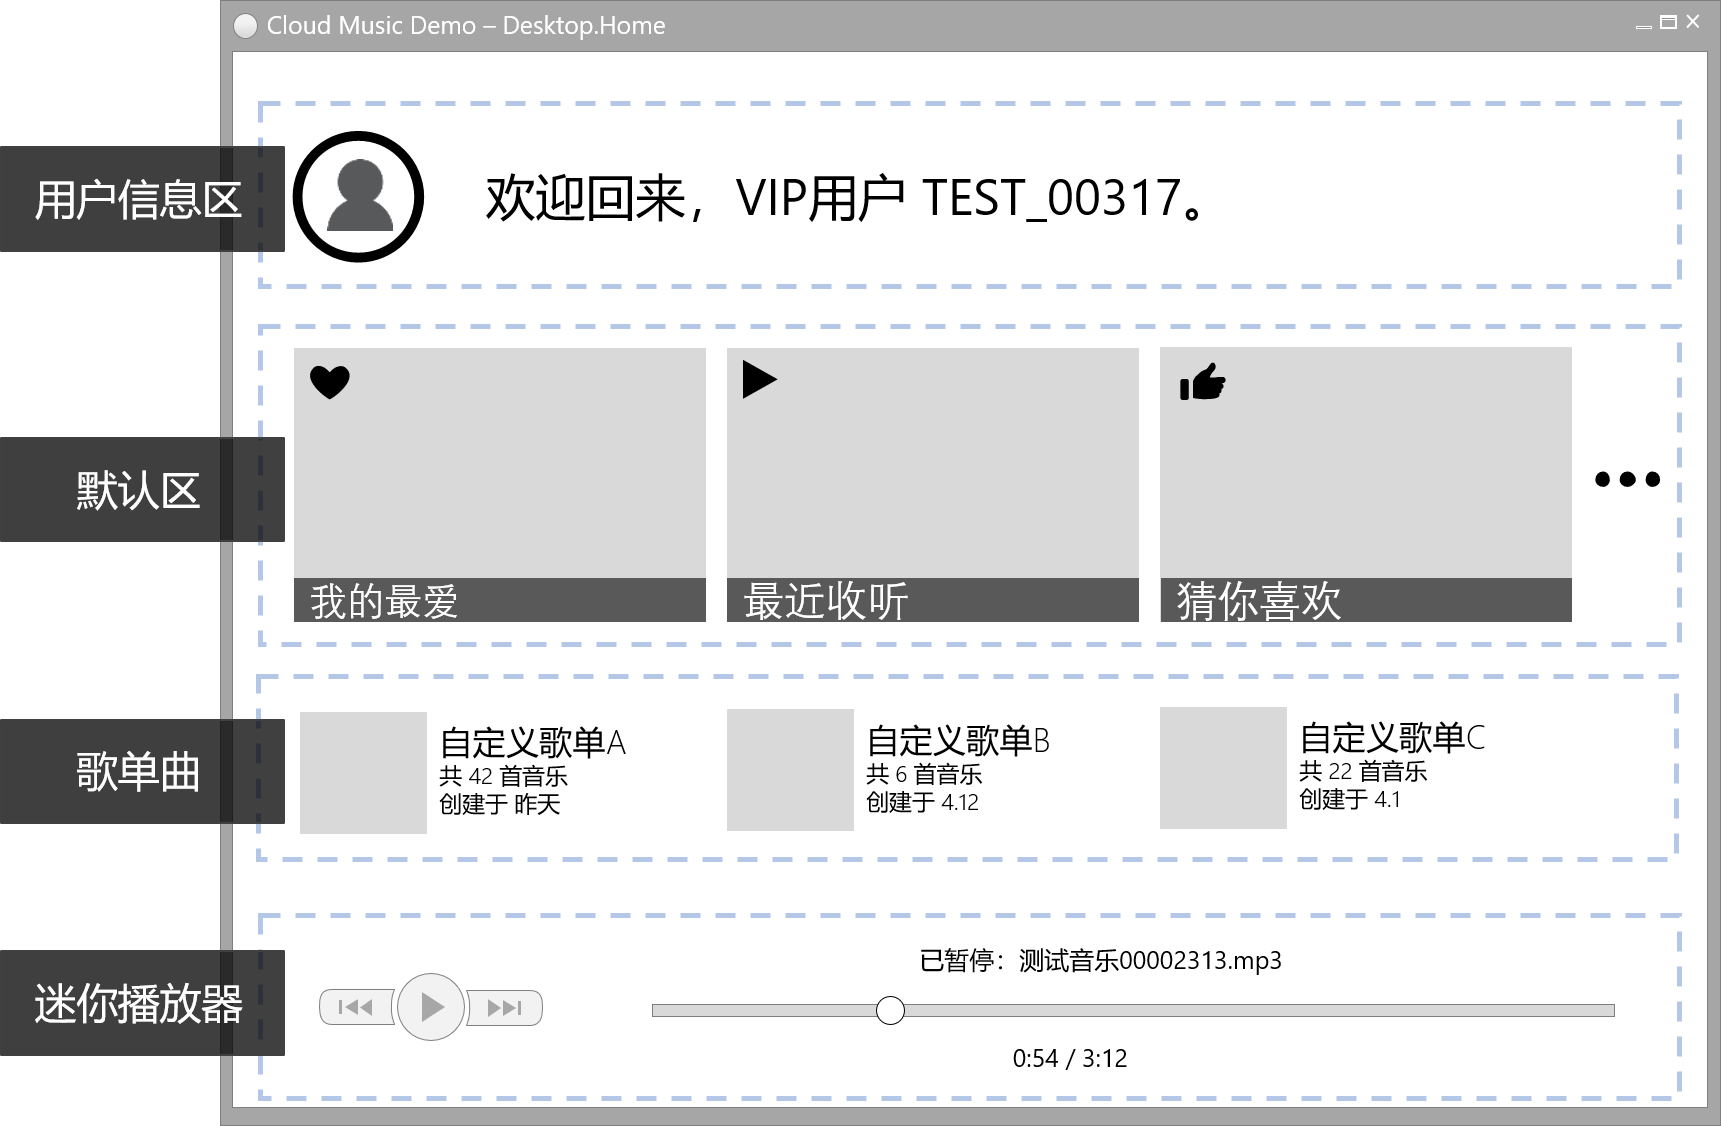
\includegraphics[width=.95\linewidth]{figures/desttop_home}

  \caption{  \label{fig:desttop_home}
  		PC客户端主页(Home Page)用户接口设计图
    }
\end{figure}

\begin{figure}[h!]
  \centering
 
  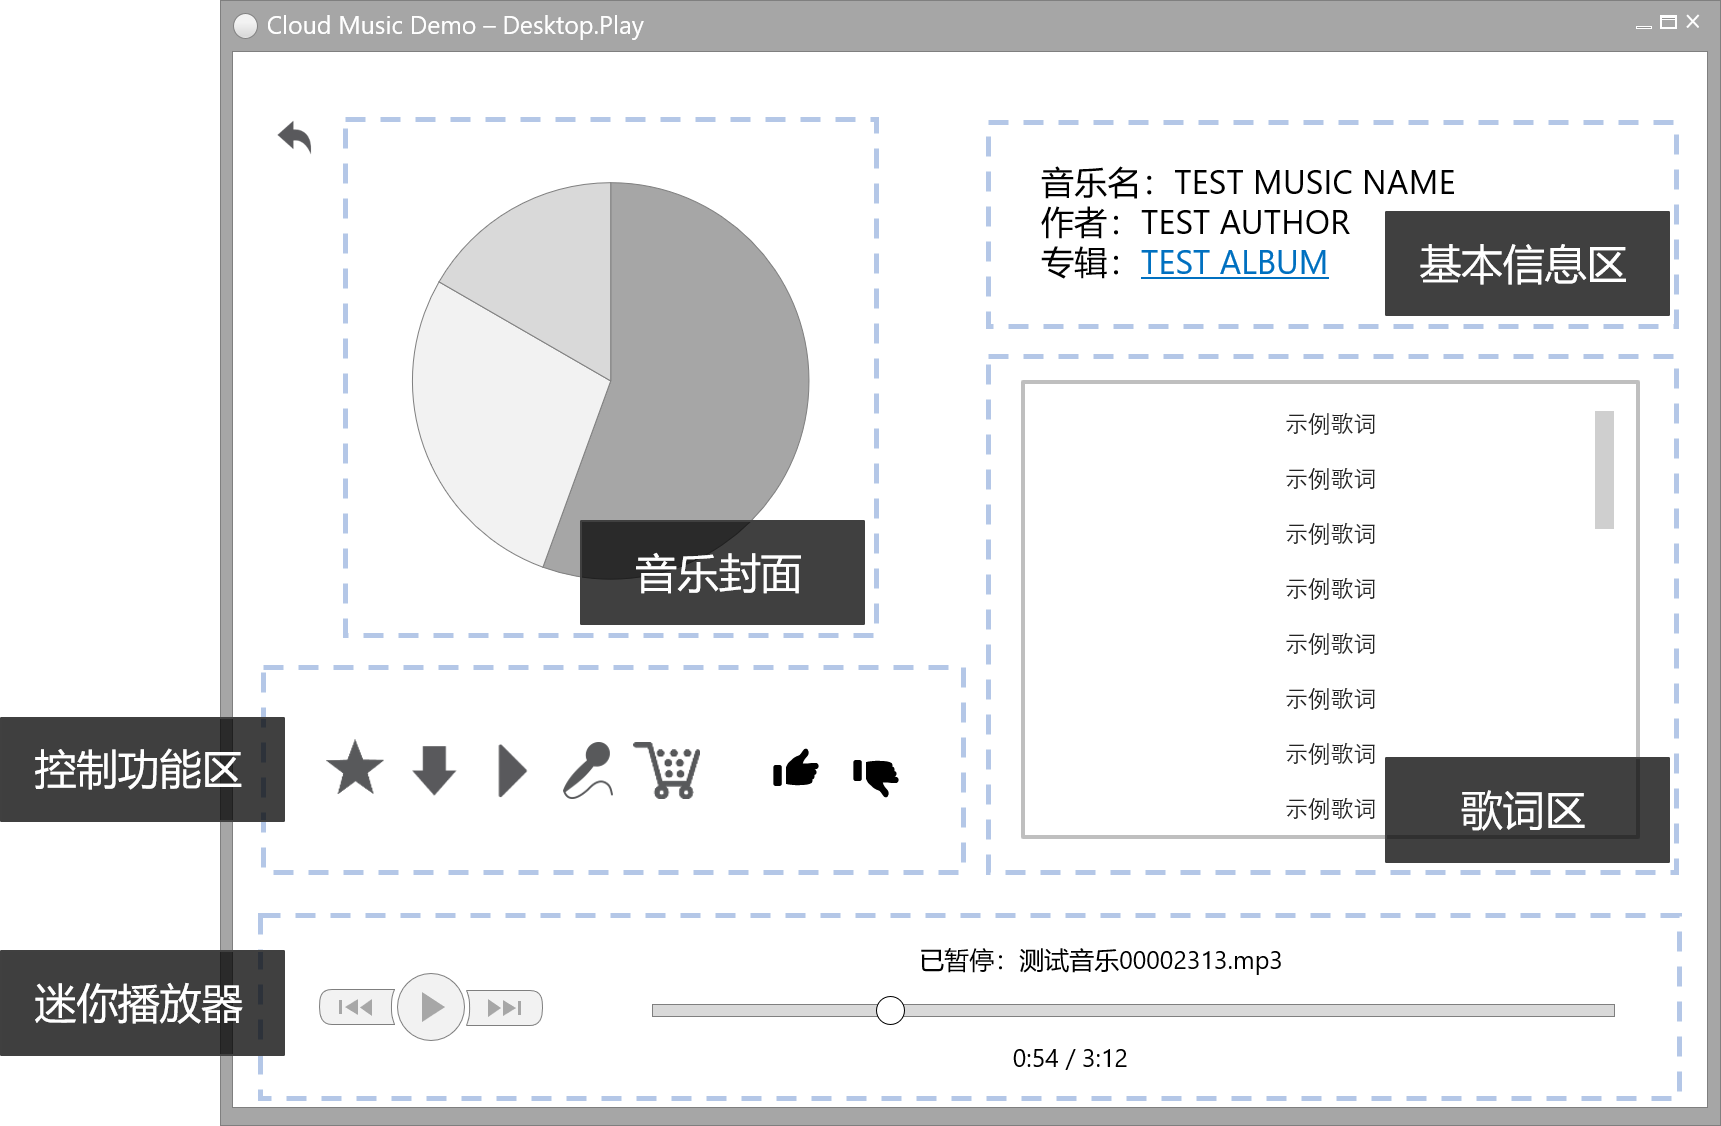
\includegraphics[width=.95\linewidth]{figures/desttop_music}

  \caption{ \label{fig:desttop_music}
  		PC客户端音乐播放界面用户接口设计图
    }
\end{figure}

\begin{figure}[h!]
  \centering

  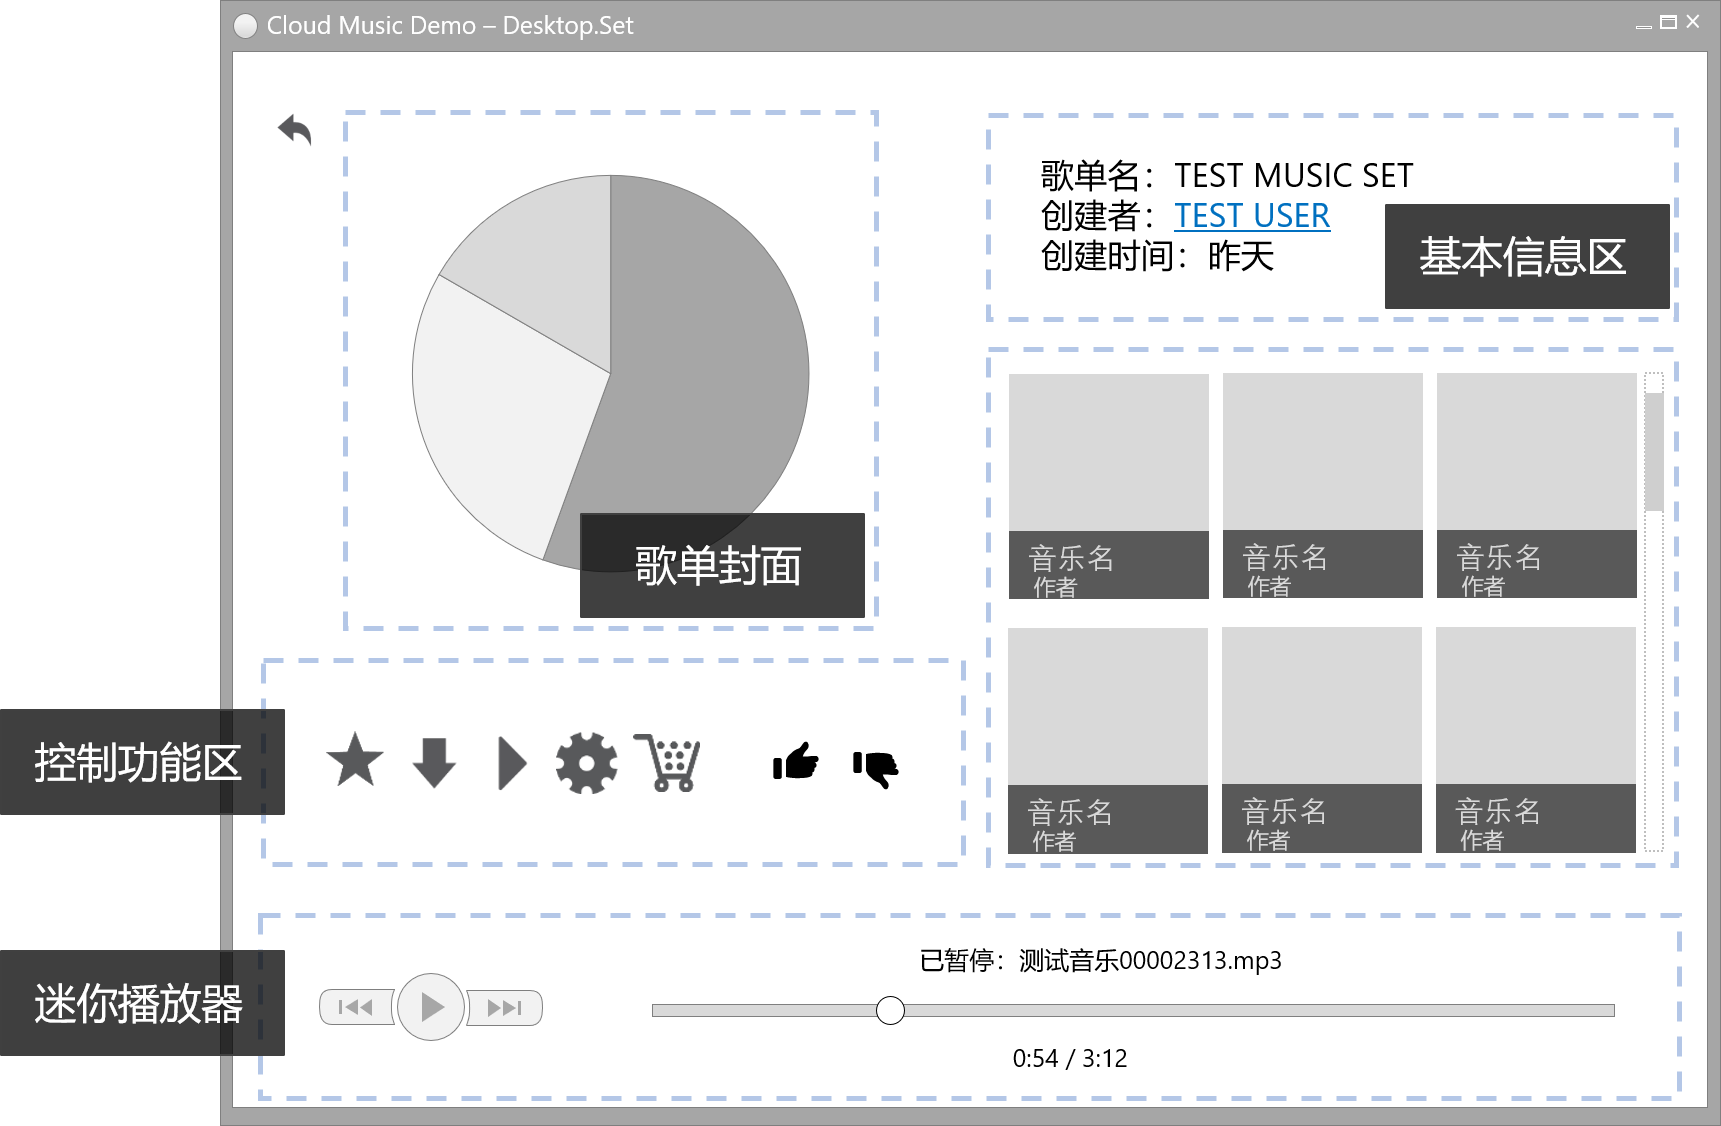
\includegraphics[width=.95\linewidth]{figures/desttop_collection}

  \caption{  \label{fig:desttop_collection}
  		PC客户端音乐集展示用户接口设计图
    }
\end{figure}


\subsubsection{移动客户端用户接口} % (fold)

\begin{enumerate}
	\item \textbf{要求的屏幕格式}:
		PC客户端支持大于$1334 \times 750$ 分辨率的移动设备屏幕,并对根据屏幕大小以及系统
		设定的屏幕元素放大比例做自动适应;
	\item \textbf{使用方式}:
		对于一般的用户,我们的产品使用逻辑与一般的移动设备软件一致,
			用户不需要主动学习便可学会使用它,
		同时,我们也会在安装后附上使用说明书,来保证用户可以方便使用;
	\item \textbf{页面规划}: 
	\begin{itemize}
		\item 主页界面的用户接口设计,请参考图\ref{fig:mobile_home};
		\item 音乐播放界面的用户接口设计,请参考图\ref{fig:mobile_music};
		\item 音乐集查看界面的用户接口设计,请参考图\ref{fig:mobile_collection};
	\end{itemize}
\end{enumerate}

\begin{figure}[h!]
  \centering

  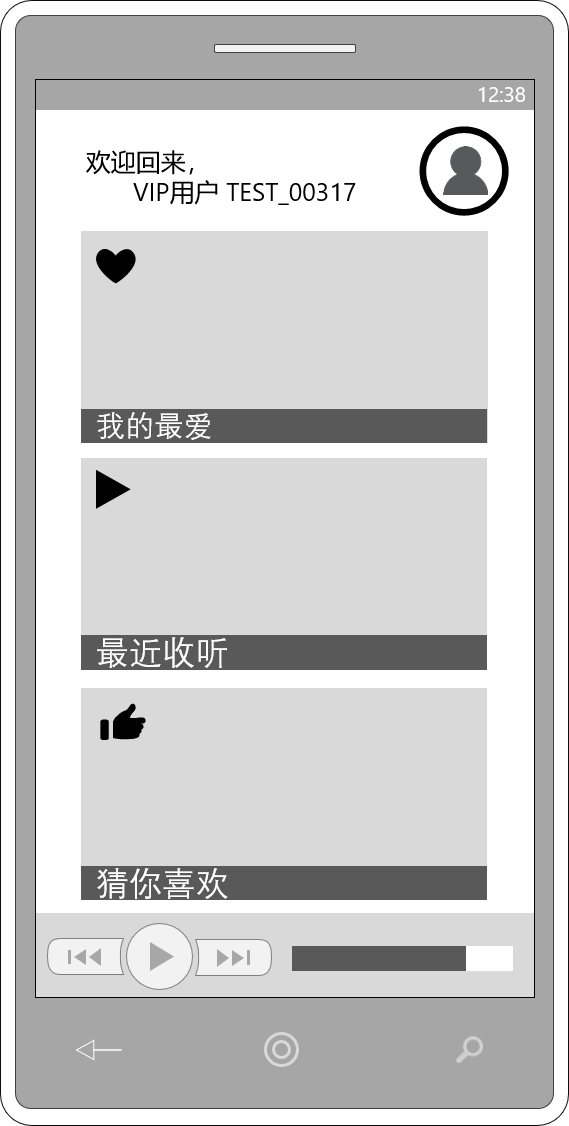
\includegraphics[width=.33\linewidth]{figures/mobile_home}

  \caption{  \label{fig:mobile_home}
  		移动客户端主页(Home Page)用户接口设计图
    }
\end{figure}

\begin{figure}[h!]
  \centering
 
  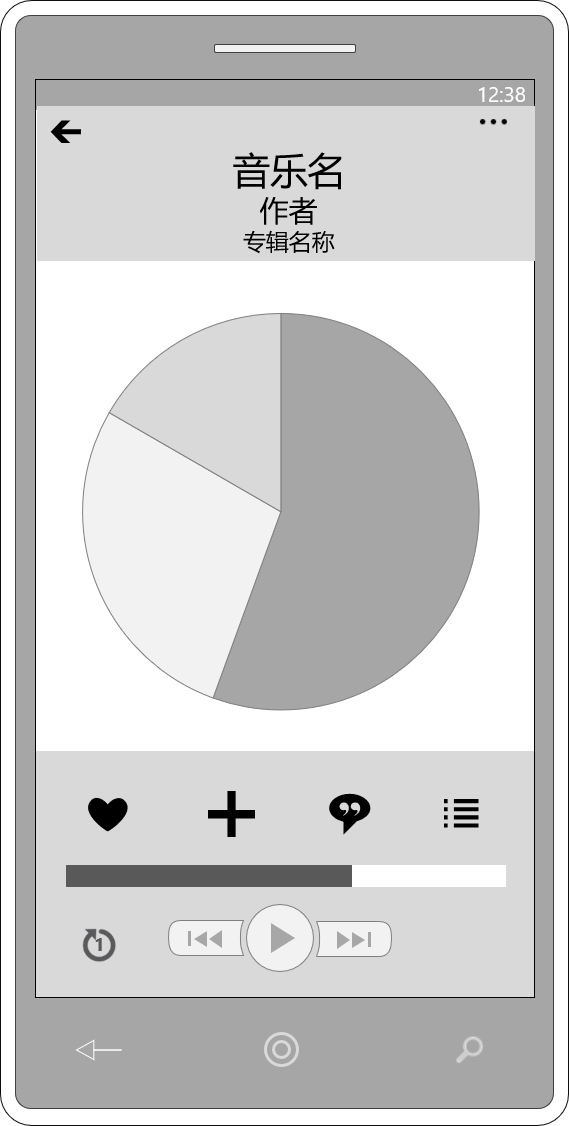
\includegraphics[width=.33\linewidth]{figures/mobile_music}

  \caption{ \label{fig:mobile_music}
  		移动客户端音乐播放界面用户接口设计图
    }
\end{figure}

\begin{figure}[h!]
  \centering

  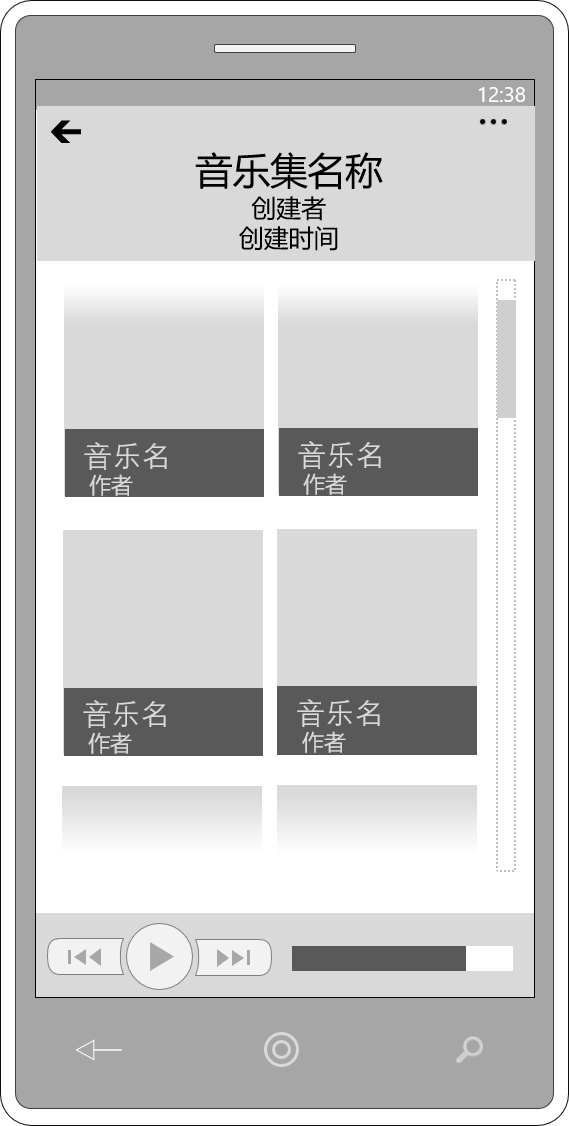
\includegraphics[width=.33\linewidth]{figures/mobile_collection}

  \caption{  \label{fig:mobile_collection}
  		移动客户端音乐集展示用户接口设计图
    }
\end{figure}


\subsubsection{网页客户端用户接口} % (fold)

\begin{enumerate}
	\item \textbf{要求的屏幕格式}:
		网页客户端支持大于$800 \times 600$ 分辨率的通用网页浏览器,
		并对根据屏幕大小以及浏览器设定的屏素放大比例做自动适应;
	\item \textbf{使用方式}:
		对于一般的用户,我们的产品使用逻辑与一般的网页一致,
			用户不需要主动学习便可学会使用它,
		同时,我们也会在安装后附上使用说明书,来保证用户可以方便使用;
	\item \textbf{页面规划}: 
	\begin{itemize}
		\item 主页界面的用户接口设计,请参考图\ref{fig:web_home};
		\item 音乐播放界面的用户接口设计,请参考图\ref{fig:web_music};
		\item 音乐集查看界面的用户接口设计,请参考图\ref{fig:web_collection};
	\end{itemize}
\end{enumerate}

\begin{figure}[h!]
  \centering

  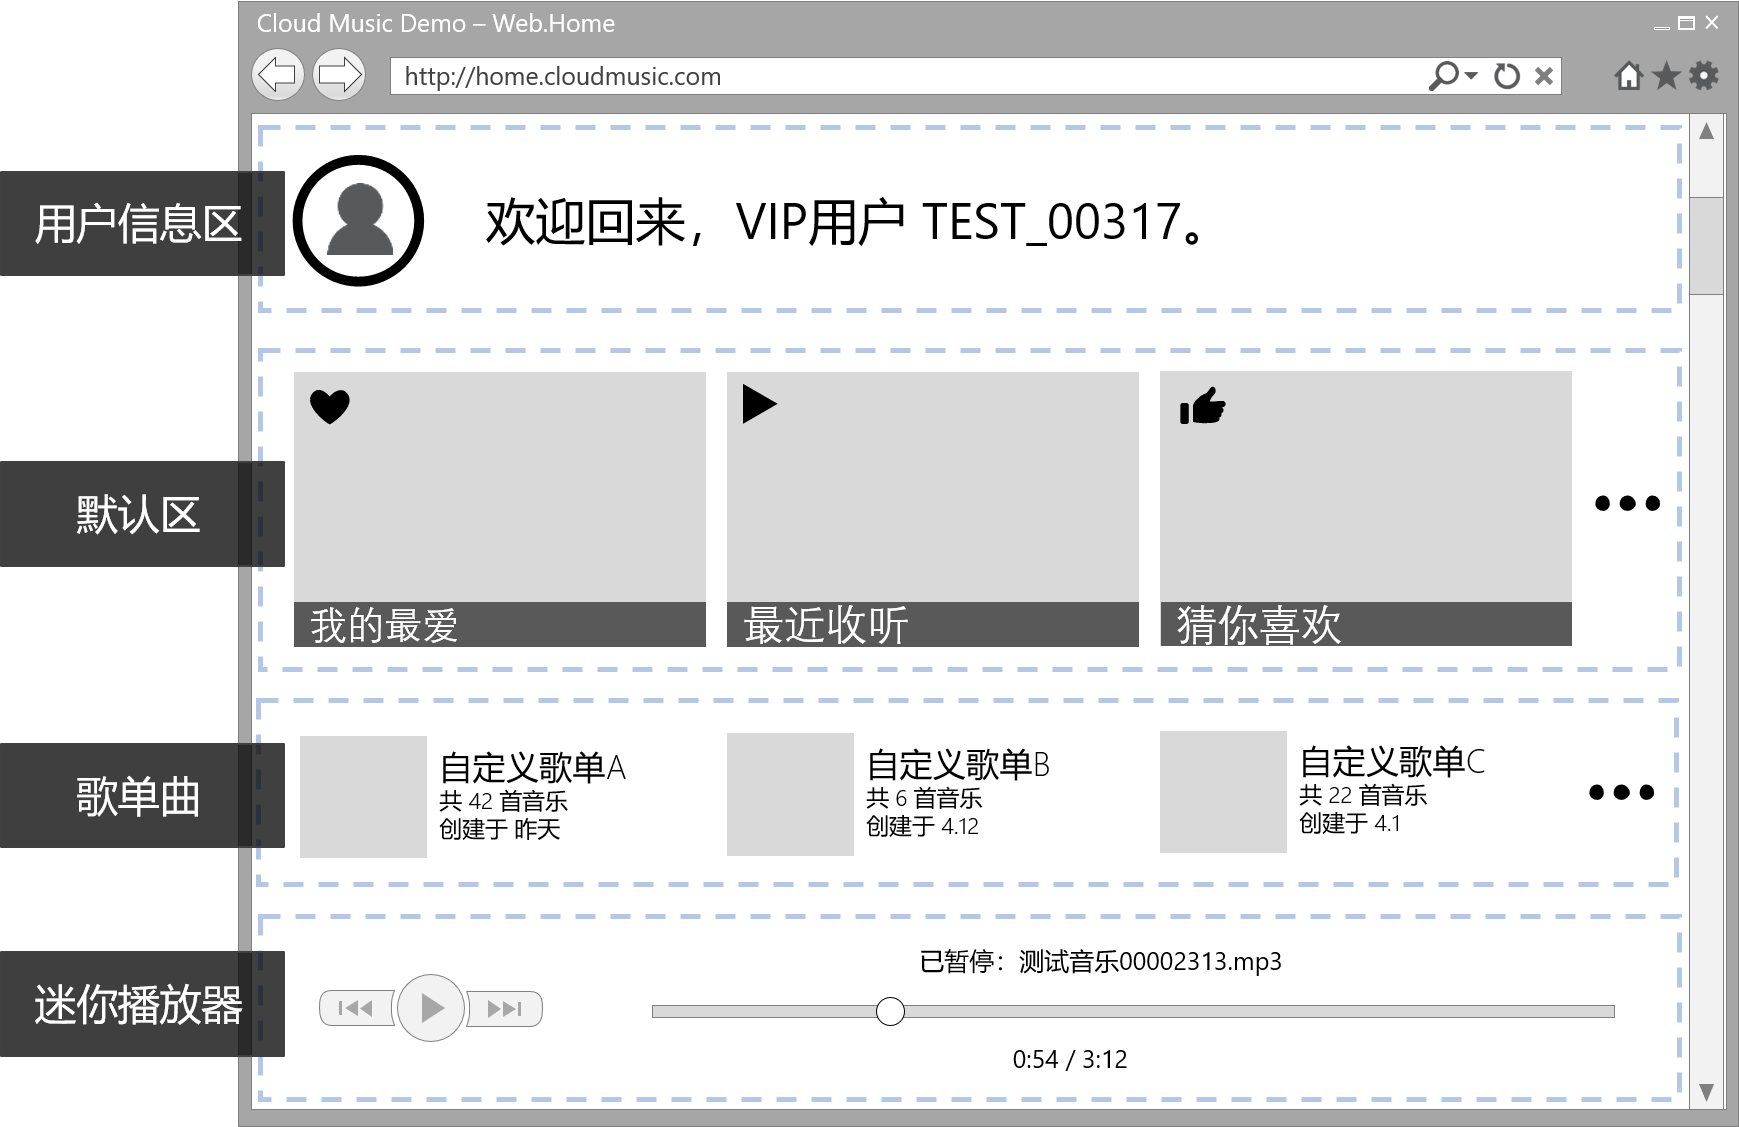
\includegraphics[width=.95\linewidth]{figures/web_home}

  \caption{  \label{fig:web_home}
  		网页客户端主页(Home Page)用户接口设计图
    }
\end{figure}

\begin{figure}[h!]
  \centering
 
  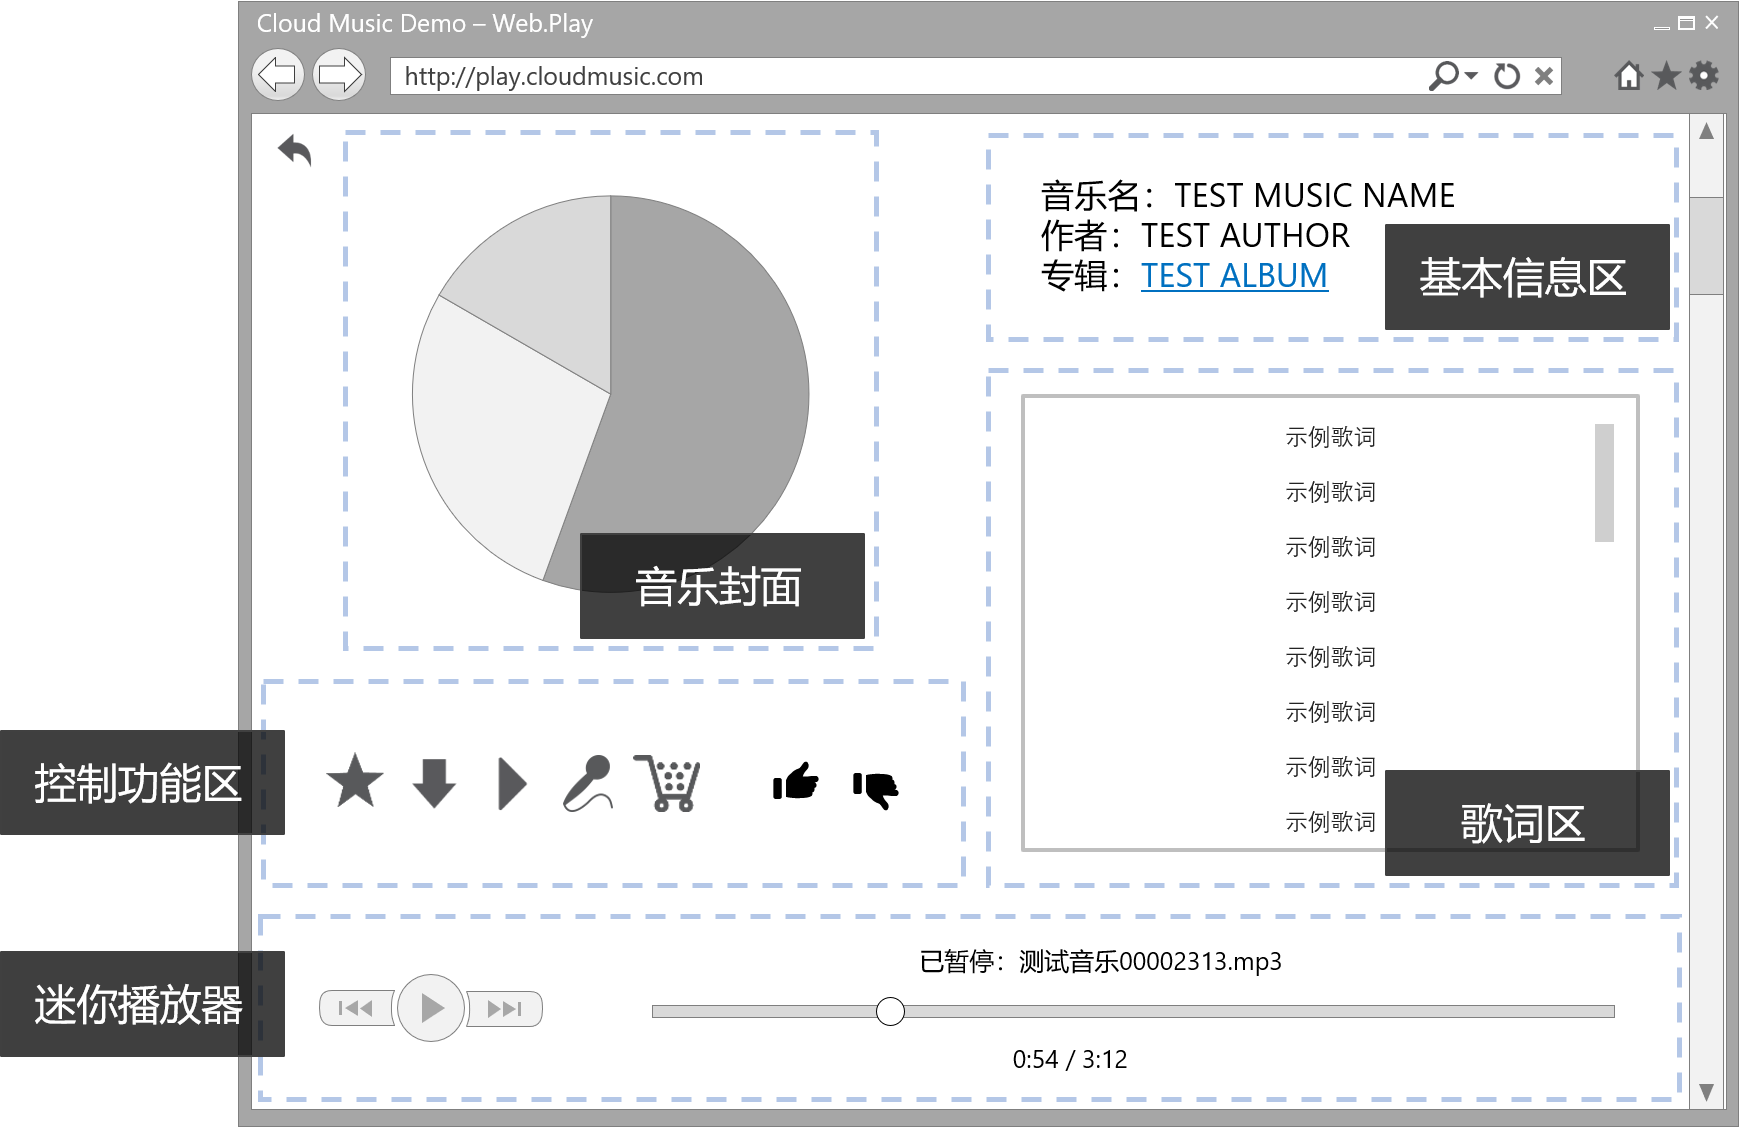
\includegraphics[width=.95\linewidth]{figures/web_music}

  \caption{ \label{fig:web_music}
  		网页客户端音乐播放界面用户接口设计图
    }
\end{figure}

\begin{figure}[h!]
  \centering

  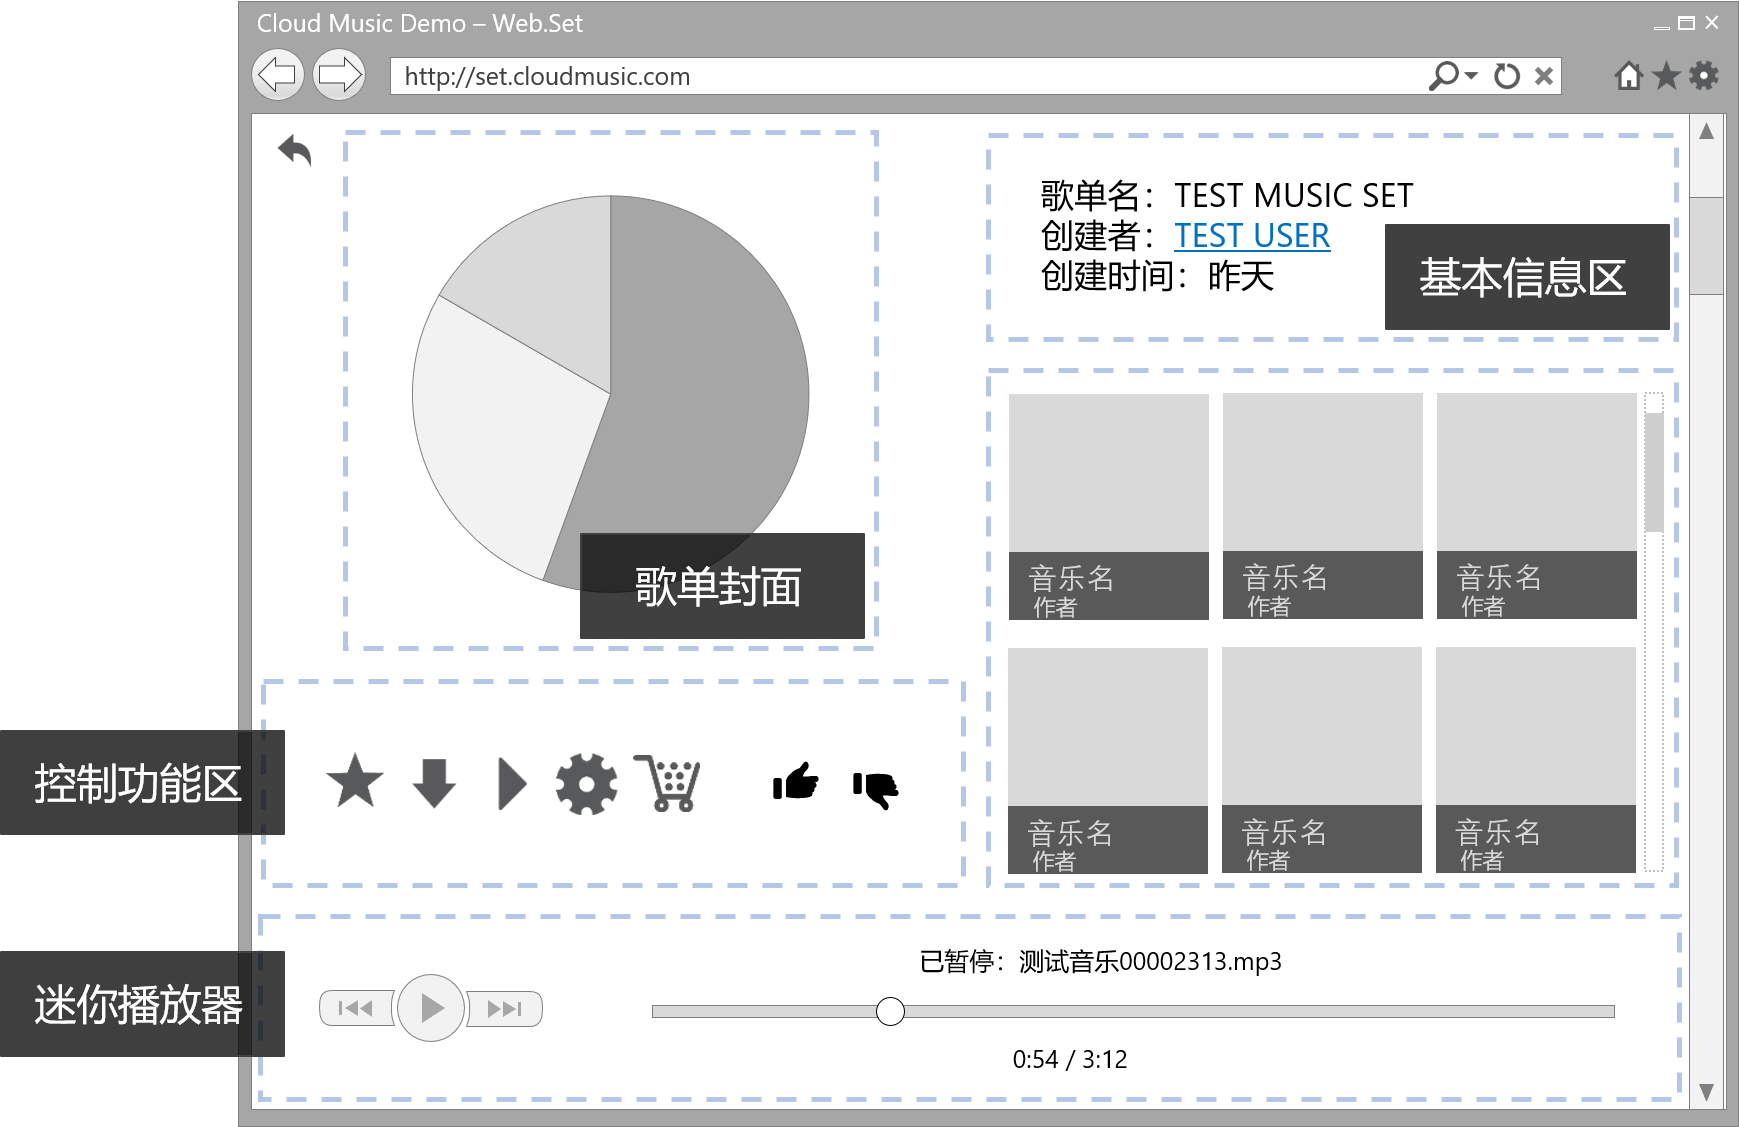
\includegraphics[width=.95\linewidth]{figures/web_collection}

  \caption{  \label{fig:web_collection}
  		网页客户端音乐集展示用户接口设计图
    }
\end{figure}



\subsection{软件接口}

\subsubsection{数据库软件产品可选项A} % (fold)
\begin{itemize}
	\item \textbf{名字}:
		Oracle Database 数据库软件
	\item \textbf{助记符}:
		Oracle Database
	\item \textbf{版本号}:
		12c Release 1
	\item \textbf{来源}:
		软件商提供的安装介质
	\item \textbf{目的}:
		作为储存服务器数据的可选项之一,我们将根据实际情况,
			最终决定是否使用它,另一选项是PostgreSQL数据库软件。
	\item \textbf{接口定义}:
		包含以下接口:
		\begin{enumerate}
			\item 查询用户 , ViewUser   , 接口格式:$\{ UID \}$
			\item 校验用户 , CheckUser  , 接口格式:$\{ UID, LoginInfo \}$
			\item 注册用户 , RegisterUser  , 接口格式:$\{ UID,  PassWord, Email\}$
			\item 查询音乐 , ViewMusic  , 接口格式:$\{ MID \}$
			\item 检验音乐可访问性 , AccessMusic ,接口格式: $\{ MID, UID, LoginInfo \}$ 
		\end{enumerate}
\end{itemize}

\subsubsection{数据库软件产品可选项B} % (fold)
\begin{itemize}
	\item \textbf{名字}:
		PostgreSQL Server
	\item \textbf{助记符}:
		PostgreSQL
	\item \textbf{版本号}:
		10.3
	\item \textbf{来源}:
		包管理器
	\item \textbf{目的}:
		作为储存服务器数据的可选项之一,我们将根据实际情况,
			最终决定是否使用它,另一选项是Oracle Database数据库软件。
	\item \textbf{接口定义}:
		包含以下接口:
		\begin{enumerate}
			\item 查询用户 , ViewUser   , 接口格式:$\{ UID \}$
			\item 校验用户 , CheckUser  , 接口格式:$\{ UID, LoginInfo \}$
			\item 注册用户 , RegisterUser  , 接口格式:$\{ UID,  PassWord, Email\}$
			\item 查询音乐 , ViewMusic  , 接口格式:$\{ MID \}$
			\item 检验音乐可访问性 , AccessMusic ,接口格式: $\{ MID, UID, LoginInfo \}$ 
		\end{enumerate}
\end{itemize}

\subsubsection{HTTP服务器} % (fold)
\begin{itemize}
	\item \textbf{名字}:
	Nginx
	\item \textbf{助记符}:
	Nginx
	\item \textbf{版本号}:
	1.14.0
	\item \textbf{来源}:
	包管理器
	\item \textbf{目的}:
	提供文件下载和动态网页的换发
	\item \textbf{接口定义}:
	使用nginx的配置文件来定义结构并过滤包,使用80和443端口对公网提供服务
\end{itemize}

\subsubsection{后端框架} % (fold)
\begin{itemize}
	\item \textbf{名字}:
	Django
	\item \textbf{助记符}:
	Django
	\item \textbf{版本号}:
	2.0.4
	\item \textbf{来源}:
	包管理器
	\item \textbf{目的}:
	提供RESTful API,运行实际服务
	\item \textbf{接口定义}:
	使用HTTP协议,监听从Nginx转发来的请求
\end{itemize}

\subsubsection{音频解码}
\begin{itemize}
	\item \textbf{名字}:
	mpg123
	\item \textbf{助记符}:
	mpg123
	\item \textbf{版本号}:
	1.25.10
	\item \textbf{来源}:
	mpg123官网: http://mpg123.org/
	\item \textbf{目的}:
	解码mp3
	\item \textbf{接口定义}:
	使用mpg123接口进行音频解码和输出
\end{itemize}

\subsection{硬件接口}

后端服务可以运行在任何32位或64位X86架构的服务器上,要求服务器有互联网接入,32GB以上的磁盘存储空间。

客户端软件要求运行在有互联网接入,有声卡的任何iOS移动设备,Android移动设备,MacOS、Windows、Linux个人计算机设备上。


\subsection{通讯接口}

使用HTTP1.0/HTTP1.1/HTTPS协议在前端和后端之间进行交互。API使用了RESTful API,利用JSON进行数据交换。

JSON所支持的数据类型如下:
\begin{itemize}
	\item \textbf{String}: 字符串
	\item \textbf{Number}: 整数或浮点数
	\item \textbf{Boolean}: 布尔类型
	\item \textbf{Array}: 数组类型
\end{itemize}

数据标记含义如下:
\begin{itemize}
	\item *必填
	\item !只读
	\item ?可选
\end{itemize}

定义扩展数据类型有:
\begin{itemize}
	\item \textbf{DateTime}: ISO-8601字符串,零时区。如 “2017-07-17T07:12:29.181605Z”
	\item \textbf{URL}: 统一资源链接,即字符串
	\item \textbf{Email}: 邮箱名,即字符串
	\item \textbf{Phone}: 电话号码,即字符串
	\item \textbf{User}: 用户信息
\begin{lstlisting}[numbers=none, frame=none]
{
    id!: Number,
    last_login!: DateTime | null,
    username!: String,
    phone_number: Phone,
    email: Email,
    description: String,
    avatar_url!: URL,
    address: String,
    description: String
}
\end{lstlisting}
	\item \textbf{Notice}: 通知
\begin{lstlisting}[numbers=none, frame=none]
{
    id!: Number,
    category!: String,
  	message!: String,
  	has_read: Boolean,
  	created!: DateTime
}
\end{lstlisting}
	\item \textbf{File}: 文件
\begin{lstlisting}[numbers=none, frame=none]
{
    id!: Number,
    file: URL,
    mime_type: String
}
\end{lstlisting}
\item \textbf{MusicQuality}: 音乐质量,可能有四个值:'128kbps'、'192kbps'、'320kbps'
\item \textbf{MusicInfo}: 音乐信息
\begin{lstlisting}[numbers=none, frame=none]
{
    name!: String,
    author!: String,
    upload_time?: DateTime,
    album_name?: String,
    music_id!: String,
}
\end{lstlisting}
\item \textbf{MusicFileInfo}: 音乐文件信息
\begin{lstlisting}[numbers=none, frame=none]
{
    quality!: MusicQuality,
    resource_url!: URL
}
\end{lstlisting}
\end{itemize}


\subsubsection{POST /api/users/username\_login/}

\noindent
功能:用户使用用户名登录\\
请求:
\begin{lstlisting}[numbers=none, frame=none]
{
    username*: String,
    password*: String,
}
\end{lstlisting}
返回:
\begin{itemize}
	\item 成功: 200 -> String = 'OK'
	\item 失败: 403 -> String // 理由
\end{itemize}

\subsubsection{POST /api/users/phone\_login/}

\noindent
功能:用户使用用户名登录\\
请求:
\begin{lstlisting}[numbers=none, frame=none]
{
   phone*: Phone,
   password*: String,
}
\end{lstlisting}
返回:
\begin{itemize}
	\item 成功: 200 -> String = 'OK'
	\item 失败: 403 -> String // 理由
\end{itemize}

\subsubsection{GET /api/users/logout/}

\noindent
功能:登出\\
返回:
\begin{itemize}
	\item 成功: 200 -> String = 'OK'
	\item 失败: 403 -> String // 理由
\end{itemize}


\subsubsection{GET /api/users/:id/}

\noindent
功能:获得:id所指示用户的信息\\
返回:
\begin{itemize}
	\item 成功: 200 -> User
	\item 未登录: 403 -> String = 'not logged'
	\item 不存在: 404
\end{itemize}



\subsubsection{POST /api/users/upload\_avatar/}

\noindent
功能:上传头像\\
请求:
\begin{lstlisting}[numbers=none, frame=none]
{
    file*: File
}
\end{lstlisting}
返回:
\begin{itemize}
	\item 成功: 200 -> String :头像的URL
	\item 未登录: 403 -> String = 'not logged'
	\item 无文件:400
\end{itemize}


\subsubsection{POST /api/users/change\_password/}

\noindent
功能:更改密码\\
请求:
\begin{lstlisting}[numbers=none, frame=none]
{
    old_pwd*: String,
    new_pwd1*: String,
    new_pwd2*: String
}
\end{lstlisting}
返回:
\begin{itemize}
	\item 成功: 200 -> String = 'OK'
	\item 未登录: 403 -> String = 'not logged'
\end{itemize}

\subsubsection{GET /api/users/reset\_password\_mail/}

\noindent
功能:向邮件发送重置链接用于重置密码\\
返回:
\begin{itemize}
	\item 成功: 200 -> String = 'OK'
	\item 请求过于频繁: 429
	\item 邮件发送失败: 500
\end{itemize}


\subsubsection{GET /api/users/reset\_password\_phone/}

\noindent
功能:向手机发送验证号码用于重置密码\\
返回:
\begin{itemize}
\item 成功: 200 -> String = 'OK'
\item 请求过于频繁: 429
\item 短信发送失败: 500
\end{itemize}



\subsubsection{GET /api/users/me/}

\noindent
功能:获得当前登录用户的信息\\
返回:
\begin{itemize}
	\item 成功: 200 -> User
	\item 未登录: 403 -> String = 'not logged'
\end{itemize}


\subsubsection{GET /api/search/:name}

\noindent
功能:对音乐名字进行搜索\\
返回:
\begin{itemize}
	\item 成功: 200 -> List<MusicInfo>
	\item 未登录: 403 -> String = 'not logged'
\end{itemize}

\subsubsection{GET /api/music/}

\noindent
功能:获得音乐文件信息\\
查询参数: qulity: MusicQuality, music\_id: String
返回:
\begin{itemize}
	\item 成功: 200 -> MusicFileInfo
	\item 未付费: 403 -> String = 'Need to buy'
	\item 未登录: 403 -> String = 'not logged'
\end{itemize}


\subsubsection{GET /api/users/add\_to\_list/}

\noindent
功能:将目标歌曲加入收听列表
查询参数: music\_id: String, list\_id: String
返回:
\begin{itemize}
	\item 成功: 200 -> String = 'OK'
	\item 未付费: 403 -> String = 'Need to buy'
	\item 未登录: 403 -> String = 'not logged'
\end{itemize}


\subsubsection{GET /api/users/delete\_from\_list/}

\noindent
功能:将目标歌曲加入收听列表
查询参数: music\_id: String, list\_id: String
返回:
\begin{itemize}
	\item 成功: 200 -> String = 'OK'
	\item 不存在歌曲: 403 -> String = 'music not found'
	\item 未登录: 403 -> String = 'not logged'
\end{itemize}

